\documentclass[10pt,landscape]{article}
\usepackage{amssymb,amsmath,amsthm,amsfonts}
\usepackage{multicol,multirow}
\usepackage{tikz}
\usepackage{pifont}
\usepackage{calc}
\usepackage{ifthen}
\usepackage{minted}
\usepackage[landscape]{geometry}
\usepackage[colorlinks=true,citecolor=blue,linkcolor=blue]{hyperref}


\ifthenelse{\lengthtest { \paperwidth = 11in}}
    { \geometry{top=.5in,left=.5in,right=.5in,bottom=.5in} }
	{\ifthenelse{ \lengthtest{ \paperwidth = 297mm}}
		{\geometry{top=1cm,left=1cm,right=1cm,bottom=1cm} }
		{\geometry{top=1cm,left=1cm,right=1cm,bottom=1cm} }
	}
\pagestyle{empty}
\makeatletter
\renewcommand{\section}{\@startsection{section}{1}{0mm}%
                                {-1ex plus -.5ex minus -.2ex}%
                                {0.5ex plus .2ex}%x
                                {\normalfont\large\bfseries}}
\renewcommand{\subsection}{\@startsection{subsection}{2}{0mm}%
                                {-1explus -.5ex minus -.2ex}%
                                {0.5ex plus .2ex}%
                                {\normalfont\normalsize\bfseries}}
\renewcommand{\subsubsection}{\@startsection{subsubsection}{3}{0mm}%
                                {-1ex plus -.5ex minus -.2ex}%
                                {1ex plus .2ex}%
                                {\normalfont\small\bfseries}}
\makeatother
\setcounter{secnumdepth}{0}
\setlength{\parindent}{0pt}
\setlength{\parskip}{0pt plus 0.5ex}
% -----------------------------------------------------------------------

\title{CPDS: LTS cheatsheet}

\begin{document}

\raggedright
\footnotesize

\begin{center}
     \Large{\textbf{CPDS: LTS cheatsheet}} \\
\end{center}
\begin{multicols}{3}
\setlength{\premulticols}{1pt}
\setlength{\postmulticols}{1pt}
\setlength{\multicolsep}{1pt}
\setlength{\columnsep}{2pt}

\section{Processes and actions}
If \textit{x} is an action and \textit{P} a process then $(x \rightarrow P$) describes a process initially engages in action $x$ and behaves as described by $P$.
\begin{verbatim}
SWITCH_ONCE = (on -> off -> STOP).
\end{verbatim}
\begin{center}
    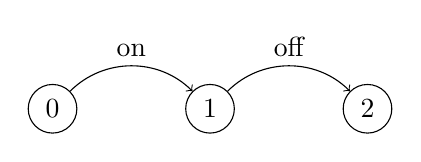
\begin{tikzpicture}
    \node[shape=circle, draw=black] at (0,0) (P0) {0};
    \node[shape=circle, draw=black] at (2,0) (P1) {1};
    \node[shape=circle, draw=black] at (4,0) (P2) {2};
    \path [->] (P0) edge[bend left=45] node[above] {on} (P1);
    \path [->] (P1) edge[bend left=45] node[above] {off} (P2);
    \end{tikzpicture}
\end{center}
\subsection{Recursion}
\begin{verbatim}
SWITCH = (on -> off -> SWITCH).
\end{verbatim}
\begin{center}
    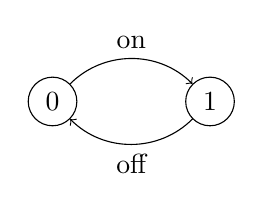
\begin{tikzpicture}
    \node[shape=circle, draw=black] at (0,0) (P0) {0};
    \node[shape=circle, draw=black] at (2,0) (P1) {1};
    \path [->] (P0) edge[bend left=45] node[above] {on} (P1);
    \path [->] (P1) edge[bend left=45] node[below] {off} (P0);
    \end{tikzpicture}
\end{center}
\section{Trace}
It represents one execution of a process.
\begin{verbatim}
on -> off -> on -> off -> on ->  off...
\end{verbatim}
\section{Choice}
Given actions $x$ and $y$ then $(x \rightarrow P| y \rightarrow Q)$ describes a process that engages in either $x$ or $y$ and adopts the behaviour of $P$ or $Q$ respectively.
\begin{verbatim}
DRINKS = ( red -> coffee -> DRINKS
        | blue -> tea -> DRINKS).
\end{verbatim}
\begin{center}
    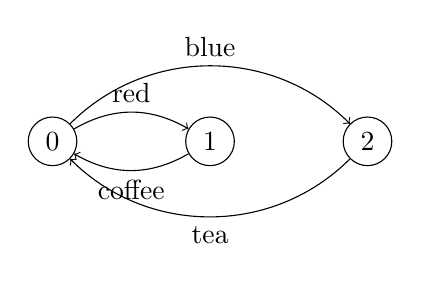
\begin{tikzpicture}
    \node[shape=circle, draw=black] at (0,0) (P0) {0};
    \node[shape=circle, draw=black] at (2,0) (P1) {1};
    \node[shape=circle, draw=black] at (4,0) (P2) {2};
    \path [->] (P0) edge[bend left=30] node[above] {red} (P1);
    \path [->] (P1) edge[bend left=30] node[below] {coffee} (P0);
    \path [->] (P0) edge[bend left=45] node[above] {blue} (P2);
    \path [->] (P2) edge[bend left=45] node[below] {tea} (P0);
    \end{tikzpicture}
\end{center}
\section{Non-deterministic choice}
Process $(x \rightarrow P | x \rightarrow Q)$ describes a process which engages in $x$ then behaves $P$ or $Q$. (Notice that the action, $x$, is the same. Which of the processes is run, $P$ or $Q$, is randomly chosen)
\begin{verbatim}
COIN = (toss -> HEADS | toss -> TAILS),
HEADS = (heads -> COIN),
TAILS = (tails -> COIN).
\end{verbatim}
\begin{center}
    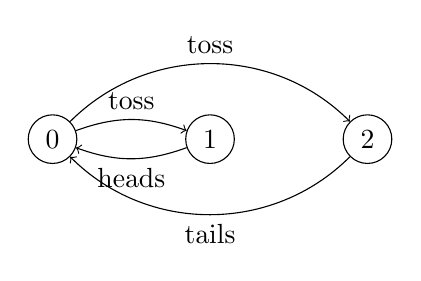
\begin{tikzpicture}
    \node[shape=circle, draw=black] at (0,0) (P0) {0};
    \node[shape=circle, draw=black] at (2,0) (P1) {1};
    \node[shape=circle, draw=black] at (4,0) (P2) {2};
    \path [->] (P0) edge[bend left=20] node[above] {toss} (P1);
    \path [->] (P1) edge[bend left=20] node[below] {heads} (P0);
    \path [->] (P0) edge[bend left=45] node[above] {toss} (P2);
    \path [->] (P2) edge[bend left=45] node[below] {tails} (P0);
    \end{tikzpicture}
\end{center}
\section{Solution to class exercise: three DAYS}
Copy the LTS code in LTSA to see the state diagrams. \\
\texttt{DAY1}: get up, then have tea, then go to work, then stop. \\
\texttt{DAY2}: do \texttt{DAY1} repeatedly. \\
\texttt{DAY3}: Do \texttt{DAY2} but choose between tea and coffee. \\
\texttt{DAY4}: Extends \texttt{DAY3} to include an \texttt{alarm} with a \texttt{snooze} button to be performed before getting up. Instead of getting up, you can snooze and go back to the start.
\begin{verbatim}
DAY1 = (up -> tea -> work -> STOP).

DAY2 = (up -> tea -> work -> DAY2).

DAY3 = (up -> DRINK),
DRINK = (tea -> WORK | coffee -> WORK),
WORK = (work -> DAY3).

DAY4 = (alarm -> ALARM),
ALARM = (up -> DRINK | snooze -> DAY4),
DRINK = (tea -> WORK | coffee -> WORK),
WORK = (work -> DAY4).
\end{verbatim}
\section{Indexed processes and actions}
The following codes are equivalent.
\begin{verbatim}
BUFF = (in[i:0..3] -> out[i] -> BUFF).

BUFF = (in[0] -> out[0] -> BUFF
        | in[1] -> out[1] -> BUFF
        | in[2] -> out[2] -> BUFF
        | in[3] -> out[3] -> BUFF).
\end{verbatim}
The parameters can be declared as \texttt{const} or \texttt{range} or as default for given processes.
\begin{verbatim}
const N = 1
range T = 0..N
range R = o..2*N

SUM = (in[a:T][b:T] -> TOTAL[a+b]),
TOTAL[s:R] = (out[s] -> SUM).

BUFF(N = 3) = (in[i:N] -> out[i] -> BUFF).
\end{verbatim}
\section{Guarded (conditional) actions}
The choice $(\textbf{when} B\text{ } x \rightarrow P \ y \rightarrow Q)$ means that $x$ is only eligible when $B$ is true.
\begin{verbatim}
COUNT(N = 3) = COUNT[0],
COUNT[i: 0..N] = (when (i < N) inc -> COUNT[i + 1]
                | when (i > 0) dec -> COUNT[i - 1]).
                
COUNTDOWN(N = 3) = (start -> COUNTDOWN[N]),
COUNTDOWN[i: 0..N] = (when (i > 0)
                        tick -> COUNTDOWN[i - 1]
                    | when (i == 0) beep -> STOP
                    | stop -> STOP).
\end{verbatim}
\begin{center}
    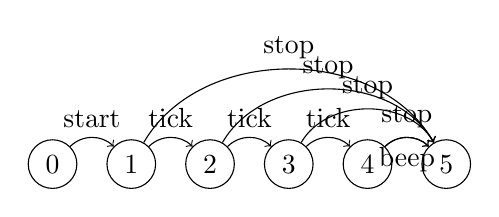
\begin{tikzpicture}
    \node[shape=circle, draw=black] at (0,0) (P0) {0};
    \node[shape=circle, draw=black] at (1,0) (P1) {1};
    \node[shape=circle, draw=black] at (2,0) (P2) {2};
    \node[shape=circle, draw=black] at (3,0) (P3) {3};
    \node[shape=circle, draw=black] at (4,0) (P4) {4};
    \node[shape=circle, draw=black] at (5,0) (P5) {5};
    \path [->] (P0) edge[bend left=45] node[above] {start} (P1);
    \path [->] (P1) edge[bend left=45] node[above] {tick} (P2);
    \path [->] (P2) edge[bend left=45] node[above] {tick} (P3);
    \path [->] (P3) edge[bend left=45] node[above] {tick} (P4);
    \path [->] (P1) edge[bend left=60] node[above] {stop} (P5);
    \path [->] (P2) edge[bend left=60] node[above] {stop} (P5);
    \path [->] (P3) edge[bend left=60] node[above] {stop} (P5);
    \path [->] (P4) edge[bend left=45] node[above] {stop} (P5);
    \path [->] (P4) edge[bend left=45] node[below] {beep} (P5);
    \end{tikzpicture}
\end{center}
\section{Solution to class exercise: SENSOR}
Model a sensor that measures the level of a tank. The level, initially 5, is measured from 0 to 9. It outputs \texttt{low} if the level is below 2, \texttt{high} if level is greater than 8, \texttt{normal} otherwise.
\begin{verbatim}
LEVEL(N=9) = SENSOR[5],
LEVEL[i:0..N] = (
        when (i < 2) low -> SENSOR[i]
        | when (i >= 2 && i < 8) normal -> SENSOR[i]
        | when (i >= 8) high -> SENSOR[i]),
SENSOR[i:0..N] = (
        when (i > 0) dec -> LEVEL[i - 1]
        | when (i < N) inc -> LEVEL[i + 1]).
\end{verbatim}
\section{Parallel composition}
For processes $P$ and $Q$, $(P||Q)$ represents the concurrent execution of $P$ and $Q$.
\begin{verbatim}
ITCH = (scratch -> STOP).
CONVERSE = (think -> talk -> STOP).
||CONVERSE_ITCH = (ITCH || CONVERSE).
\end{verbatim}
The previous code permits any of the following traces:\\
\texttt{think->talk->scratch}\\
\texttt{think->scratch->talk}\\
\texttt{scratch->think->talk}
\section{Shared actions}
If processes have actions in common, these actions are said to be shared. These must be executed at the same time by all processes that share it.
\begin{verbatim}
MAKER = (make -> ready -> MAKER).
USER = (ready -> use -> USER).
||MAKER_USER = (MAKER || USER).
\end{verbatim}
In the example above, the user can't \texttt{use} until the action \texttt{ready} happens. This can only happen after action \texttt{make}. Also, if \texttt{make} happens a second time, \texttt{ready} can not happen if the user has not \texttt{used} yet. This is, all concurrent processes must be synchronized in an action before the shared action for it to happen.
\begin{center}
    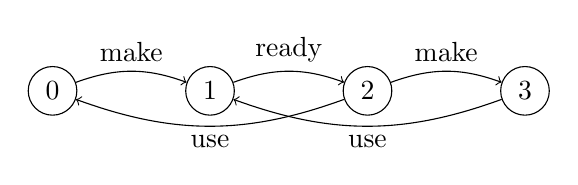
\begin{tikzpicture}
    \node[shape=circle, draw=black] at (0,0) (P0) {0};
    \node[shape=circle, draw=black] at (2,0) (P1) {1};
    \node[shape=circle, draw=black] at (4,0) (P2) {2};
    \node[shape=circle, draw=black] at (6,0) (P3) {3};
    \path [->] (P0) edge[bend left=20] node[above] {make} (P1);
    \path [->] (P1) edge[bend left=20] node[above] {ready} (P2);
    \path [->] (P2) edge[bend left=20] node[above] {make} (P3);
    \path [->] (P2) edge[bend left=20] node[below] {use} (P0);
    \path [->] (P3) edge[bend left=20] node[below] {use} (P1);
    \end{tikzpicture}
\end{center}
\subsection{Handshake}
\begin{verbatim}
MAKERv2 = (make -> ready -> used -> MAKERv2).
USERv2 = (ready -> use -> used -> USERv2).
||MAKER_USERv2 = (MAKERv2 || USERv2).
\end{verbatim}
This code prevents the maker from keeping working if the thing it has made has not yet been used. Concurrent processes are forced to be synchronized. This is the handshake.
\begin{center}
    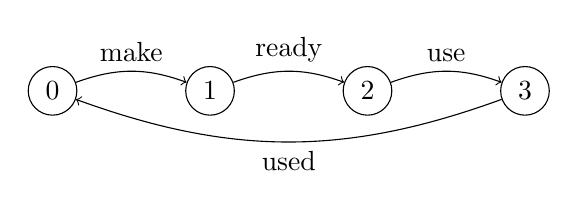
\begin{tikzpicture}
    \node[shape=circle, draw=black] at (0,0) (P0) {0};
    \node[shape=circle, draw=black] at (2,0) (P1) {1};
    \node[shape=circle, draw=black] at (4,0) (P2) {2};
    \node[shape=circle, draw=black] at (6,0) (P3) {3};
    \path [->] (P0) edge[bend left=20] node[above] {make} (P1);
    \path [->] (P1) edge[bend left=20] node[above] {ready} (P2);
    \path [->] (P2) edge[bend left=20] node[above] {use} (P3);
    \path [->] (P3) edge[bend left=20] node[below] {used} (P0);
    \end{tikzpicture}
\end{center}
\section{Class exercise: \texttt{||MICROWAVE}}
Model the \texttt{MICROWAVE} using parallel composition, via handshaking with shared actions.
\begin{verbatim}
COOK = (put_food_in -> cook -> take_food_out -> COOK).
SET_HEAT = (put_food_in -> set_heat ->
        cook -> SET_HEAT).
SET_TIME = (put_food_in -> set_time ->
        cook -> SET_TIME).

||MICROWAVE = (COOK || SET_HEAT || SET_TIME).
\end{verbatim}
Actually, the previous code forces you to put the food in before you can set the time and heat. We assume that is intended.
\section{Process relabelling}
Label $a:P$ gives one of the processes $P$ the name $a$.
\begin{verbatim}
SWITCH = (on -> off -> SWITCH).
||TWO_SWITCH = (toilet:SWITCH || kitchen:SWITCH).
\end{verbatim}
Processes can be labelled as an instance in an array.
\begin{verbatim}
||SWITCHES(N = 3) = (s[i:1..N]:SWITCH).
\end{verbatim}
Finally, processes can be labelled by a set of prefix labels. \texttt{\{a1,...,ax\}::P} replaces every action label $n$ with the labels \texttt{a1.n,...,ax.n}. For every transition $(n\rightarrow X)$ is replaced with transitions $(\{a1.n,...,ax.n\}\rightarrow X)$.
\section{Class exercise: \texttt{RESOURCE\_SHARE}}
As an example of the prefix labels, see code below:
\begin{verbatim}
RESOURCE = (acquire -> release -> RESOURCE).
USER = (acquire -> use -> release -> USER).
||RESOURCE_SHARE = (a:USER || b:USER
                || {a,b}::RESOURCE).
\end{verbatim}
This translates to two independently operating users that share a resource.
\begin{center}
    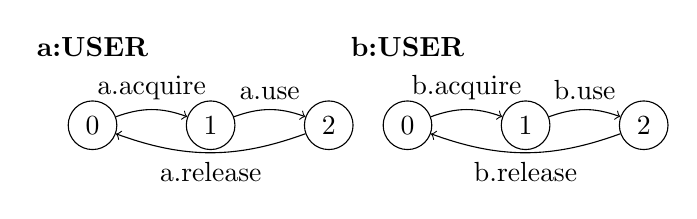
\begin{tikzpicture}
    \node[] at (0,0) {\textbf{a:USER}};
    \node[] at (4,0) {\textbf{b:USER}};
    \node[shape=circle, draw=black] at (0,-1) (P0) {0};
    \node[shape=circle, draw=black] at (1.5,-1) (P1) {1};
    \node[shape=circle, draw=black] at (3,-1) (P2) {2};
    \path [->] (P0) edge[bend left=20] node[above] {a.acquire} (P1);
    \path [->] (P1) edge[bend left=20] node[above] {a.use} (P2);
    \path [->] (P2) edge[bend left=20] node[below] {a.release} (P0);
    \node[shape=circle, draw=black] at (4,-1) (P00) {0};
    \node[shape=circle, draw=black] at (5.5,-1) (P01) {1};
    \node[shape=circle, draw=black] at (7,-1) (P02) {2};
    \path [->] (P00) edge[bend left=20] node[above] {b.acquire} (P01);
    \path [->] (P01) edge[bend left=20] node[above] {b.use} (P02);
\path [->] (P02) edge[bend left=20] node[below] {b.release} (P00);
    \end{tikzpicture}
\end{center}
\begin{center}
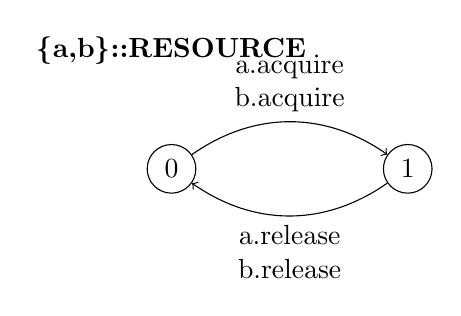
\begin{tikzpicture}
\node[] at (0,0) {\textbf{\{a,b\}::RESOURCE}};
    \node[shape=circle, draw=black] at (0,-1.5) (P0) {0};
    \node[shape=circle, draw=black] at (3,-1.5) (P1) {1};
    \path [->] (P0) edge[bend left=35] node[align=center, above] {a.acquire \\ b.acquire} (P1);
    \path [->] (P1) edge[bend left=35] node[align=center, below] {a.release \\ b.release} (P0);
    \end{tikzpicture}
\end{center}
The solution to the exercise would be the following LTS graph.
\begin{center}
    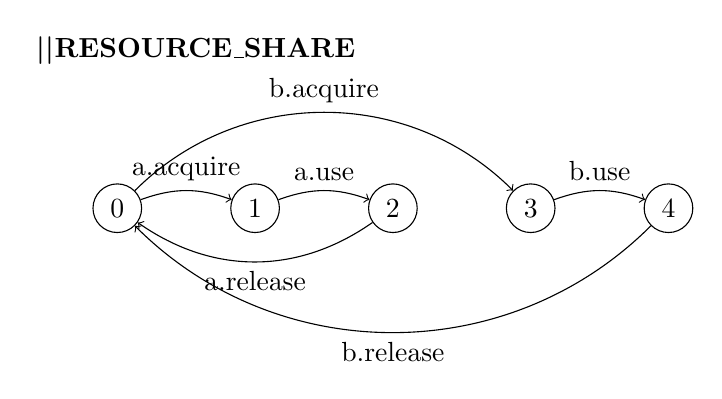
\begin{tikzpicture}
    \node[] at (0,0) {\textbf{\textbar \textbar RESOURCE\_SHARE}};
    \node[shape=circle, draw=black] at (-1,-2) (P0) {0};
    \node[shape=circle, draw=black] at (0.75,-2) (P1) {1};
    \node[shape=circle, draw=black] at (2.5,-2) (P2) {2};
    \node[shape=circle, draw=black] at (4.25,-2) (P3) {3};
    \node[shape=circle, draw=black] at (6,-2) (P4) {4};
    \path [->] (P0) edge[bend left=20] node[above] {a.acquire} (P1);
    \path [->] (P1) edge[bend left=20] node[above] {a.use} (P2);
    \path [->] (P2) edge[bend left=35] node[below] {a.release} (P0);
    \path [->] (P0) edge[bend left=45] node[above] {b.acquire} (P3);
    \path [->] (P3) edge[bend left=20] node[above] {b.use} (P4);
    \path [->] (P4) edge[bend left=45] node[below] {b.release} (P0);
    \end{tikzpicture}
\end{center}
\section{Action relabelling}
Relabelling functions are applied to processes to change the names of action labels. It goes by the format \texttt{/\{newlabel\_1 / oldlabel\_1, ..., newlabel\_n / oldlabel\_n\}}.
\begin{verbatim}
CLIENT = (call -> wait -> continue -> CLIENT).
SERVER = (request -> service -> reply -> SERVER).
||CLIENT_SERVER = (CLIENT || SERVER) / {call / request,
                                        reply / wait}.
\end{verbatim}
In this context, action \texttt{call} equals action \texttt{request} and action \texttt{reply} equals action \texttt{wait}. As can be seen on the animator, calling the action on the left hand side of the relabelling (\texttt{call} and \texttt{reply} in this case) will trigger the action on the right hand side (\texttt{request} and \texttt{wait}).
\begin{center}
    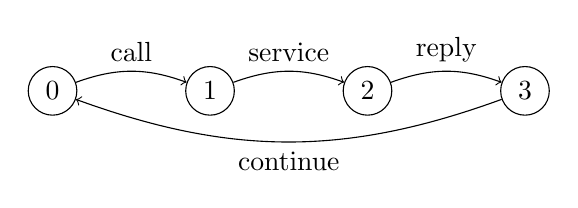
\begin{tikzpicture}
    \node[shape=circle, draw=black] at (0,0) (P0) {0};
    \node[shape=circle, draw=black] at (2,0) (P1) {1};
    \node[shape=circle, draw=black] at (4,0) (P2) {2};
    \node[shape=circle, draw=black] at (6,0) (P3) {3};
    \path [->] (P0) edge[bend left=20] node[above] {call} (P1);
    \path [->] (P1) edge[bend left=20] node[above] {service} (P2);
    \path [->] (P2) edge[bend left=20] node[above] {reply} (P3);
    \path [->] (P3) edge[bend left=20] node[below] {continue} (P0);
    \end{tikzpicture}
\end{center}
\section{Action hiding}
Hides an action $x$ from process $P$ alphabet. These actions still happen but silently. They are labelled \texttt{tau} and can not be shared between processes.
\begin{verbatim}
USER = (acquire -> use -> release -> USER) \{use}.
\end{verbatim}
Hidden actions can be run using the \texttt{step} or \texttt{run} buttons in the animator.
\begin{center}
    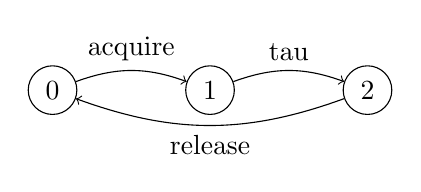
\begin{tikzpicture}
    \node[shape=circle, draw=black] at (0,0) (P0) {0};
    \node[shape=circle, draw=black] at (2,0) (P1) {1};
    \node[shape=circle, draw=black] at (4,0) (P2) {2};
    \path [->] (P0) edge[bend left=20] node[above] {acquire} (P1);
    \path [->] (P1) edge[bend left=20] node[above] {tau} (P2);
    \path [->] (P2) edge[bend left=20] node[below] {release} (P0);
    \end{tikzpicture}
\end{center}
Minimized equivalent LTS graph:
\begin{center}
    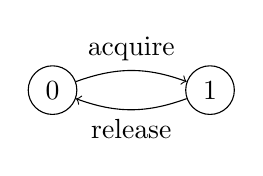
\begin{tikzpicture}
    \node[shape=circle, draw=black] at (0,-1.5) (P0) {0};
    \node[shape=circle, draw=black] at (2,-1.5) (P1) {1};
    \path [->] (P0) edge[bend left=20] node[above] {acquire} (P1);
    \path [->] (P1) edge[bend left=20] node[below] {release} (P0);
    \end{tikzpicture}
\end{center}
\section{Class exercise: \texttt{||FACTORY}}
\begin{verbatim}
MAKER_A = (make_A -> ready -> restart -> MAKER_A).
MAKER_B = (make_B -> ready -> restart -> MAKER_B).
ASSEMBLER_A_B = (ready -> assemble_A_B -> ready_two
                -> ASSEMBLER_A_B).
ASSEMBLER = (ready_two -> make_C -> assemble_A_B_C
                -> output -> restart -> ASSEMBLER).
||FACTORY = (MAKER_A || MAKER_B || ASSEMBLER_A_B 
            || ASSEMBLER)
            \{ready, ready_two}.
\end{verbatim}
Let's review all the concepts of LTS that coincide in this code. \texttt{ready} and \texttt{ready\_two} are hidden actions and will be shown as \texttt{tau} in the LTS graph. They are also shared actions, just like \texttt{restart}. This means that this will run as follows: \\
From the beginning, it is possible to choose between \texttt{make\_A} and \texttt{make\_B}. After both comes hidden \texttt{ready}, so it means that, regardless of the order, both \texttt{make} actions must happen before. After \texttt{ready}, action \texttt{restart} from processes \texttt{MAKER\_A} and \texttt{MAKER\_B} can not be run until other processes reach it, as it is a shared action. \\
Now only \texttt{ASSEMBLER\_A\_B} is allowed to run the action \texttt{assemble\_A\_B}, which will allow hidden action \texttt{ready\_two}. Process \texttt{ASSEMBLER\_A\_B} can now begin again. \\
After action \texttt{ready\_two}, process \texttt{ASSEMBLER} can run actions \texttt{assemble\_A\_B\_C} and \texttt{output}, which will allow both \texttt{MAKER} processes and itself to run action \texttt{restart} and start again.\\
This is represented in the following graph:
\begin{center}
    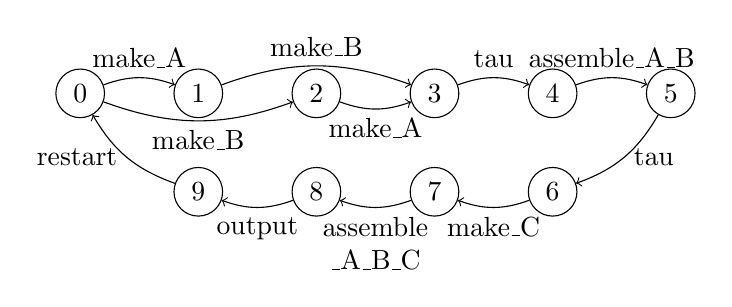
\begin{tikzpicture}
    \node[shape=circle, draw=black] at (0,0) (P0) {0};
    \node[shape=circle, draw=black] at (1.5,0) (P1) {1};
    \node[shape=circle, draw=black] at (3,0) (P2) {2};
    \node[shape=circle, draw=black] at (4.5,0) (P3) {3};
    \node[shape=circle, draw=black] at (6,0) (P4) {4};
    \node[shape=circle, draw=black] at (7.5,0) (P5) {5};
    \node[shape=circle, draw=black] at (6,-1.25) (P6) {6};
    \node[shape=circle, draw=black] at (4.5,-1.25) (P7) {7};
    \node[shape=circle, draw=black] at (3,-1.25) (P8) {8};
    \node[shape=circle, draw=black] at (1.5,-1.25) (P9) {9};
    \path [->] (P0) edge[bend left=20] node[above] {make\_A} (P1);
    \path [->] (P0) edge[bend right=20] node[below] {make\_B} (P2);
    \path [->] (P1) edge[bend left=20] node[above] {make\_B} (P3);
    \path [->] (P2) edge[bend right=20] node[below] {make\_A} (P3);
    \path [->] (P3) edge[bend left=20] node[above] {tau} (P4);
    \path [->] (P4) edge[bend left=20] node[above] {assemble\_A\_B} (P5);
    \path [->] (P5) edge[bend left=20] node[right] {tau} (P6);
    \path [->] (P6) edge[bend left=20] node[below] {make\_C} (P7);
    \path [->] (P7) edge[bend left=20] node[align=center, below] {assemble \\ \_A\_B\_C} (P8);
    \path [->] (P8) edge[bend left=20] node[below] {output} (P9);
    \path [->] (P9) edge[bend left=20] node[left] {restart} (P0);
    \end{tikzpicture}
\end{center}
The minimized version is:
\begin{center}
    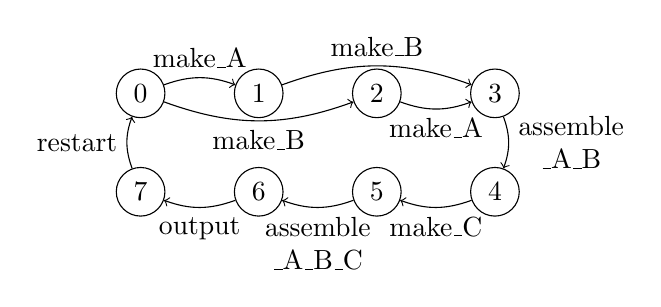
\begin{tikzpicture}
    \node[shape=circle, draw=black] at (0,0) (P0) {0};
    \node[shape=circle, draw=black] at (1.5,0) (P1) {1};
    \node[shape=circle, draw=black] at (3,0) (P2) {2};
    \node[shape=circle, draw=black] at (4.5,0) (P3) {3};
    \node[shape=circle, draw=black] at (4.5,-1.25) (P4) {4};
    \node[shape=circle, draw=black] at (3,-1.25) (P5) {5};
    \node[shape=circle, draw=black] at (1.5,-1.25) (P6) {6};
    \node[shape=circle, draw=black] at (0,-1.25) (P7) {7};
    \path [->] (P0) edge[bend left=20] node[above] {make\_A} (P1);
    \path [->] (P0) edge[bend right=20] node[below] {make\_B} (P2);
    \path [->] (P1) edge[bend left=20] node[above] {make\_B} (P3);
    \path [->] (P2) edge[bend right=20] node[below] {make\_A} (P3);
    \path [->] (P3) edge[bend left=20] node[align=center, right] {assemble \\ \_A\_B} (P4);
    \path [->] (P4) edge[bend left=20] node[below] {make\_C} (P5);
    \path [->] (P5) edge[bend left=20] node[align=center, below] {assemble \\ \_A\_B\_C} (P6);
    \path [->] (P6) edge[bend left=20] node[below] {output} (P7);
    \path [->] (P7) edge[bend left=20] node[left] {restart} (P0);
    \end{tikzpicture}
\end{center}
\section{Correctness}
Let $S$ be a sequential program. \\
Formula $\{P\}S\{Q\}$ is \textbf{partially correct} if every terminating computation of $S$ that starts in state $P$ terminates in state $Q$. (Does not mean all will terminate, but the ones that do will do it satisfying $Q$) \\
$\{P\}S\{Q\}$ is \textbf{totally correct} if every computation in $S$ starts in state $P$ and terminate in state $Q$. (All computations terminate, and all will end satisfying $Q$).\\
$P$ is the precondition and $Q$ the postcondition.
\section{Safety}
\subsection{\texttt{CONVOY} and \texttt{CARS} model}
\begin{verbatim}
const N = 3
range ID = 1..N

CAR = (enter -> exit -> CAR).

NOPASS1 = C_ENTER[1],
C_ENTER[i:ID] = ([i].enter -> C_ENTER[i % N + 1]).

NOPASS2 = C_EXIT[1],
C_EXIT[i:ID] = ([i].exit -> C_EXIT[i % N + 1]).

||CONVOY = ([ID]:CAR || NOPASS1 || NOPASS2).

||CARS = (red:CONVOY || blue:CONVOY).
\end{verbatim}
The model above defines a car process that goes through actions \texttt{enter} and \texttt{exit}. \texttt{N} amount of cars are created per convoy with \texttt{[ID]:CAR}, which are identified by numbers from 1 to \texttt{N}, including the latter. This code equals \texttt{(1:CAR || 2:CAR || 3:CAR || ...)}. \\
Both \texttt{NOPASS} processes start off as \texttt{C[1]} \footnote{In the slides, \texttt{NOPASS1} and \texttt{NOPASS2} both initialize a homonym process \texttt{C[1]}. The two \texttt{C} processes are actually different despite their shared names and each works only within the scope of the bigger process, delimited by the dot (\texttt{.}). To avoid confusion, they have been renamed for the example}. This makes the first of a convoy the only one able to move. Moreover, actions \texttt{enter} and \texttt{exit} are shared across \texttt{[i]:CAR} and \texttt{C[i]}. This means that at the beginning, only \texttt{[1].enter} can be run, which will enable \texttt{[1].exit}, which will enable the next car to follow the same process, and so on. This is, this code does not allow overtaking. \\
Two concurrent convoys are created but no safety is implemented as to permitting traffic in only one way.
\subsection{\texttt{BRIDGE} model}
\begin{verbatim}
BRIDGE = BRIDGE[0][0],
BRIDGE[nRed:T][nBlue:T] =
    (when (nBlue == 0)
        red[ID].enter -> BRIDGE[nRed + 1][nBlue]
    | red[ID].exit -> BRIDGE[nRed - 1][nBlue]
    | when (nRed == 0)
        blue[ID].enter -> BRIDGE[nRed][nBlue + 1]
    | blue[ID].exit -> BRIDGE[nRed][nBlue - 1]).
\end{verbatim}
The \texttt{BRIDGE} processes starts the bridge as empty, no car of any color is passing through. Its function is to count the amount of cars of each type on the bridge, allowing only cars of either. \\
Notice that the \texttt{when} clause only applies to the \texttt{enter} actions. This means that \texttt{exit} actions permit car counts to decrease below 0.
\subsection{Safety properties}
A safety property $P$ defines a deterministic process that asserts that any trace in the alphabet of $P$ is accepted by $P$. Those actions that are not part of the specified behaviour of $P$ are transitions to the error state. \\
Unrelated example.
\begin{verbatim}
property POLITE = (knock -> enter -> POLITE).
\end{verbatim}
\begin{center}
    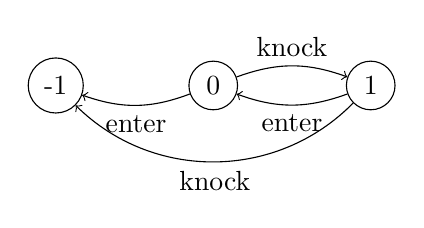
\begin{tikzpicture}
    \node[shape=circle, draw=black] at (0,0) (P-1) {-1};
    \node[shape=circle, draw=black] at (2,0) (P0) {0};
    \node[shape=circle, draw=black] at (4,0) (P1) {1};
    \path [->] (P0) edge[bend left=20] node[above] {knock} (P1);
    \path [->] (P1) edge[bend left=20] node[below] {enter} (P0);
    \path [->] (P0) edge[bend left=20] node[below] {enter} (P-1);
    \path [->] (P1) edge[bend left=45] node[below] {knock} (P-1);
    \end{tikzpicture}
\end{center}
Possible traces:
\begin{itemize}
    \item \texttt{knock} $\rightarrow$ \texttt{enter} \ding{51}
    \item \texttt{enter} \ding{55}
    \item \texttt{knock} $\rightarrow$ \texttt{knock} \ding{55}
\end{itemize}
Applied to the single lane problem.
\begin{verbatim}
property ONEWAY = (red[ID].enter -> RED[1]
        | blue[ID].enter -> BLUE[1]),
RED[i:ID] = (red[ID].enter -> RED[i+1]
        | when (i == 1) red[ID].exit -> ONEWAY
        | when (i > 1) red[ID].exit -> RED[i - 1]),
BLUE[i:ID] = (blue[ID].enter -> BLUE[i+1]
        | when (i == 1) blue[ID].exit -> ONEWAY
        | when (i > 1) blue[ID].exit -> BLUE[i - 1]).
        
||SingleLaneBridge = (CARS || BRIDGE || ONEWAY).
\end{verbatim}
The addition of this safety property means that each time \texttt{ONEWAY} is reached the next action can only lead to either \texttt{RED[1]} or \texttt{BLUE[1]}. Anything else would trigger an error state.
\section{Class exercise: \texttt{SUPERMARKET}}
\begin{verbatim}
const Min = 1
const Max = 3
SHELF = BOT[0],
BOT[i:0..Max] = (when (i > 0) get[k:1..i] -> BOT[i-k]
				| when (i <= Min) fill -> BOT[Max]).

WORKER = (fill -> WORKER).

CLIENT = (get[1..Max] -> CLIENT).

||SUPERMARKET = (SHELF || WORKER || CLIENT).
\end{verbatim}
Below, the LTS graph. For convenience, the number on the nodes represent the amount of bottles on the shelf.
\begin{center}
    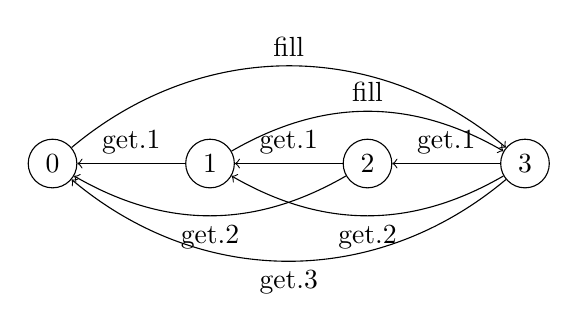
\begin{tikzpicture}
    \node[shape=circle, draw=black] at (0,0) (P0) {0};
    \node[shape=circle, draw=black] at (2,0) (P1) {1};
    \node[shape=circle, draw=black] at (4,0) (P2) {2};
    \node[shape=circle, draw=black] at (6,0) (P3) {3};
    \path [->] (P0) edge[bend left=40] node[above] {fill} (P3);
    \path [->] (P1) edge[bend left=30] node[above] {fill} (P3);
    \path [->] (P1) edge[] node[align=center, above] {get.1} (P0);
    \path [->] (P2) edge[] node[align=center, above] {get.1} (P1);
    \path [->] (P3) edge[] node[align=center, above] {get.1} (P2);
    \path [->] (P3) edge[bend left=30] node[align=center, below] {get.2} (P1);
    \path [->] (P2) edge[bend left=30] node[align=center, below] {get.2} (P0);
    \path [->] (P3) edge[bend left=40] node[align=center, below] {get.3} (P0);
    \end{tikzpicture}
\end{center}
\section{Liveness}
A liveness property asserts that something good eventually happens.
\section{Progress}
A progress property $P = \{a1,...,an\}$ asserts that it in an infinite execution of a target system, at least one of the actions $\{a1,...,an\}$ will be executed infinitely often.
\subsection{Fair choice}
If a choice over a set of transitions is executed infinitely often, then every transition in the set will be executed infinitely often.
\begin{verbatim}
COIN = (toss -> heads -> COIN
        | toss -> tails -> COIN).
\end{verbatim}
If a coin is tossed an infinite number of times, we would expect that heads would be chosen infinitely often and that tails would be chosen infinitely often. These progress properties assure that is the case:
\begin{verbatim}
progress HEADS = {heads}
progress TAILS = {tails}
\end{verbatim}
On the other hand, if the same progress properties were added to the code given below, the progress property \texttt{TAILS} could not be fulfilled.
\begin{verbatim}
TWOCOIN =  (pick -> COIN | pick -> TRICK),
TRICK = (toss -> heads -> TRICK),
COIN = (toss -> heads -> COIN | toss -> tails -> COIN).
\end{verbatim}
This is because for an infinite amount of executions, and given the non-deterministic nature of the process, \texttt{tails} is not able to execute infinitely often, because one of the coins will never give tails.\\
Going back to the single lane bridge problem.
\begin{verbatim}
progress BLUECROSS = {blue[ID].enter}
progress REDCROSS = {red[ID].enter}
\end{verbatim}
These progress properties aim to guarantee that blue cars enter (therefore end up crossing) infinitely often and red cars too. But it is possible to loop through the same type of cars: Enter one blue car, then another one, then the first exits, then a third enters. This would not be detected as progress violations.\\
This is because fair choice means that eventually every possible execution will occur, including those in which cars do not starve.
\subsection{Action priority}
Action priority expresions describe scheduling properties.
\subsubsection{High priority}
High priority specifies a composition in which actions $\{a1,...,an\}$ have higher priority than any other action in the process.
\begin{verbatim}
||C = (P || Q) << {a1, ..., an}
\end{verbatim}
\subsubsection{Low priority}
Low priority specifies a composition in which actions $\{a1,...,an\}$ have lower priority than any other action in the process.
\begin{verbatim}
||C = (P || Q) >> {a1, ..., an}
\end{verbatim}
Both types of priority work by finding out which of the choices in the system include actions labeled by any of the labels included in the priority expressions. The lower priority ones (which could be actions $\{a1,...,an\}$ marked as low priority or regular actions in comparison to high priority ones) are discarded.
\subsubsection{Example}
\begin{verbatim}
NORMAL = (work -> play -> NORMAL
        | sleep -> play -> NORMAL).
||HIGH = (NORMAL) << {work}.
||LOW = (NORMAL) >> {work}.
\end{verbatim}
The code above would result in the LTS graphs below. Notice the differences.
\begin{center}
    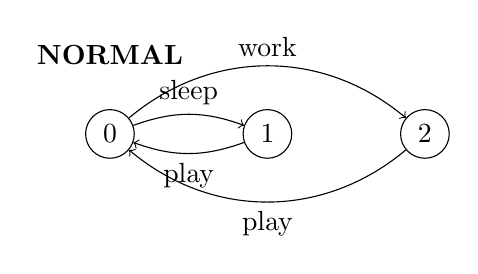
\begin{tikzpicture}
    \node[] at (0,0) {\textbf{NORMAL}};
    \node[shape=circle, draw=black] at (0,-1) (P0) {0};
    \node[shape=circle, draw=black] at (2,-1) (P1) {1};
    \node[shape=circle, draw=black] at (4,-1) (P2) {2};
    \path [->] (P0) edge[bend left=20] node[above] {sleep} (P1);
    \path [->] (P1) edge[bend left=20] node[below] {play} (P0);
    \path [->] (P0) edge[bend left=40] node[above] {work} (P2);
    \path [->] (P2) edge[bend left=40] node[below] {play} (P0);
    \end{tikzpicture}
\end{center}
\begin{center}
    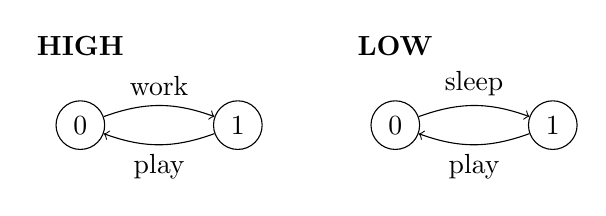
\begin{tikzpicture}
    \node[] at (0,0) {\textbf{HIGH}};
    \node[shape=circle, draw=black] at (0,-1) (P0) {0};
    \node[shape=circle, draw=black] at (2,-1) (P1) {1};
    \path [->] (P0) edge[bend left=20] node[above] {work} (P1);
    \path [->] (P1) edge[bend left=20] node[below] {play} (P0);
    \node[] at (4,0) {\textbf{LOW}};
    \node[shape=circle, draw=black] at (4,-1) (P0) {0};
    \node[shape=circle, draw=black] at (6,-1) (P1) {1};
    \path [->] (P0) edge[bend left=20] node[above] {sleep} (P1);
    \path [->] (P1) edge[bend left=20] node[below] {play} (P0);
    \end{tikzpicture}
\end{center}
\section{Sources}
\href{https://www.doc.ic.ac.uk/~jnm/book/slides.html}{Slides by Magee \& Kramer}
\vfill
\hrule
~\\
Unai Perez Mendizabal \textcopyright \href{https://github.com/unaipme}{https://github.com/unaipme}
\end{multicols}
\newpage
\begin{center}
     \Large{\textbf{CPDS: Erlang cheatsheet}} \\
\end{center}
\begin{multicols}{3}
You can run all the examples of this sheet with the Erlang shell (command \texttt{erl}).
\section{Variables}
Variables in Erlang start with a capital letter and are actually constant. Once assigned they can not be changed.
\begin{minted}[breaklines]{erlang}
1> X = 123456789.
123456789
2> X.
123456789
3> X = 1234.
** exception error: no match of right hand sidevalue 1234
\end{minted}
All statements end with a point (\texttt{.}).
\begin{minted}{erlang}
4> X * X
4> .
15241578750190521
\end{minted}
\section{Atoms}
An atom is a literal, a constant with a name. Has no value by itself but can be used as a value.
\begin{minted}{erlang}
1> foo.
foo
2> bar.
bar
\end{minted}
They must start with a lower case letter and can not have other characters than alphanumeric characters, underscores (\texttt{\_}) or @, unless they are enclosed in single quotes.
\begin{minted}{erlang}
3> Length.
* 1: variable 'Length' is unbound
4> 'Length'.
'Length'
5> foo_bar@.
foo_bar@.
6> foo bar.
* 1: syntax error before: bar
\end{minted}
\section{Tuples}
A single entity that groups a fixed amount of items is a tuple. It is analog to an object from OOP.
\subsection{Creating tuples}
\begin{minted}[breaklines]{erlang}
1> FirstName = {firstName, joe}.
{firstName, joe}
2> LastName = {lastName, armstrong}.
{lastName, armstrong}
3> Person = {person, FirstName, LastName}.
{person,{firstName, joe},{lastName, armstrong}}
\end{minted}
\subsection{Reading from tuples}
\begin{minted}{erlang}
1> Point = {point, 10, 45}.
{point,10,45}
\end{minted}
Given the \texttt{Point} variable created above, the numeric values can be extracted as follows:
\begin{minted}{erlang}
2> {point, X, Y} = Point.
{point,10,45}
3> X.
10
4> Y.
45
\end{minted}
Recall variables start with capital letter and atoms with lowercase. This means that, while \texttt{X} and \texttt{Y} are being used to store the values of the tuple, \texttt{point} is being used as a placeholder for pattern matching. The following line of code will not work:
\begin{minted}[breaklines]{erlang}
5> {foo, X1, Y1} = point.
** exception error: no match of right hand side value {point,10,45}
\end{minted}
\section{Anonymous variable}
If we are not interested in using atoms or pattern matching, certain part of the tuple's content can be discarded using the underscore (\texttt{\_}) as anonymous variable. \\
Given the \texttt{Person} tuple created in the previous section, we can read the last name like this:
\begin{minted}{erlang}
4> {_, {_, Name}, _} = Person.
{person,{firstName,joe},{lastName,armstrong}}
5> Name.
joe
\end{minted}
Notice the underscore represents \textit{something} we do not care about. The first two times it is used in the previous example, it is a placeholder for an atom. The third time, it is a placeholder for a whole tuple.
\section{Functions and modules}
An example on how to work with Erlang from outside the shell. We create a file with the following content:
\begin{minted}[breaklines]{erlang}
-module(geometry).
-export([area/1]).
area({rectangle, Width, Height}) -> Width * Height;
area({circle, R}) -> 3.14159 * R * R.
\end{minted}
\texttt{-module(<name>)} defines the name of the module that will include the functions declared in the file. The name must be the same as that of the file. With \texttt{-export([])}, we declare what functions we want to be accessible from outside the module itself (kind of like the \texttt{public} keyword in Java). Functions are listed in format \texttt{[name1/numArgs1,...]}, which permits the exportation of functions based on their name and the argument amount. \\
If a function receives multiple implementations, which is the case, these must be delimited by a semicolon (\texttt{;}), except for the last one, which must end with a point (\texttt{.}). \\
This definitely means that both implementations of \texttt{area} will be exported because both of them have just one argument. These arguments are in both cases tuples that allow for pattern matching as explained before: clauses beginning with lowercase are atom literals, and actual parameters otherwise. \\
The module can now be loaded and used like this:
\begin{minted}{erlang}
1> c(geometry).
{ok,geometry}
2> geometry:area({rectangle, 10, 5}).
50
3> geometry:area({circle, 1.4}).
6.15752
\end{minted}
\section{Class exercise: \texttt{weekDay}}
\begin{minted}[breaklines]{erlang}
-module(dates).
-export([classify_day/1]).

classify_day(monday) -> weekDay;
classify_day(tuesday) -> weekDay;
classify_day(wednesday) -> weekDay;
classify_day(thursday) -> weekDay;
classify_day(friday) -> weekDay;
classify_day(saturday) -> weekEnd;
classify_day(sunday) -> weekEnd.
\end{minted}
Saved it as a file named \texttt{dates.erl} and opened a shell session in the same directory. Can be used as follows:
\begin{minted}[breaklines]{erlang}
1> c(dates).
{ok,dates}
2> dates:classify_day(monday).
weekDay
3> dates:classify_day(saturday).
weekEnd
4> dates:classify_day(april).   
** exception error: no function clause matching dates:classify_day(april) (dates.erl, line 4)
\end{minted}
\section{Class exercise: Factorial}
\begin{minted}[breaklines]{erlang}
-module(myfactorial).
-export([factorial/1]).

factorial(0) -> 1;
factorial(1) -> 1;
factorial(N) -> N * factorial(N - 1).
\end{minted}
Notice that the least generic parameter definitions must be first, otherwise they will never be reached. For example, if \texttt{factorial(N)} was the first implementation, none of the other implementations would ever be run, because when calling \texttt{factorial(0)} it will get matched with \texttt{factorial(N)} before it gets the chance to match none of the others. \\
The file is saved as \texttt{myfactorial.erl}. Execution example:
\begin{minted}{erlang}
1> c(myfactorial)
{ok,myfactorial}
2> myfactorial:factorial(5).
120
\end{minted}
\section{Concurrency basics}
\subsection{\texttt{spawn}}
Creates a new concurrent process that runs the given function. Returns the process ID (PID), which can be used to send messages between processes.
\begin{minted}{erlang}
Pid = spawn(Fun).
\end{minted}
\subsection{Message passing}
By using the PID of the newly created concurrent process, we can send messages to it.
\begin{minted}{erlang}
Pid ! Message.
\end{minted}
\subsection{Message reception}
Messages passed using the previous method can be received with the keyword \texttt{receive}.
\begin{minted}{erlang}
receive
    Pattern1 [when Condition1] -> Expression1;
    ...
    PatternN [when ConditionN] -> ExpressionN;
Other -> OtherExpression
end.
\end{minted}
\section{Concurrency example}
\begin{minted}[breaklines]{erlang}
-module(area_server0).
-export([loop/0]).

loop() ->
  receive
    {rectangle, Width, Height} ->
      io:format("Area of rectangle is ~p~n", [Width * Height]),
      loop();
    {circle, R} ->
      io:format("Area of circle is ~p~n", [3.14159 * R * R]),
      loop();
    Other ->
      io:format("The shape ~p is unknown~n", [Other]),
      loop()
  end.
\end{minted}
How to run it:
\begin{minted}{erlang}
1> c(area_server0).
{ok,area_server0}
2> Pid = spawn(fun area_server0:loop/0).
<0.67.0>
3> Pid ! {nothing}.
The shape {nothing} is unknown
{nothing}
4> Pid ! {circle, 5}.
Area of circle is 78.53975
{circle,5}
5> Pid ! {rectangle, 5, 8}.
Area of rectangle is 40
{rectangle,5,8}
\end{minted}
\subsection{Client-server}
Notice that, even though the output of the spawned process can be seen, there is no direct interaction between the parent and child processes. The client-server paradigm implies the interaction between a client, which is responsible of starting the communication, and a server. This can be emulated in Erlang by passing the PID along with the message we send to the server:
\begin{minted}[breaklines]{erlang}
-module(area_server1).
-export([loop/0, rpc/2]).

rpc(Pid, Request) -> 
  Pid ! {self(), Request},
  receive ->
    Response -> Response
  end.

loop() ->
  receive
    {From, {rectangle, Width, Height}} ->
      From ! Width * Height,
      loop();
    {From, {circle, R}} ->
      From ! 3.14159 * R * R,
      loop();
    {From, Other} ->
      From ! {error, Other},
      loop()
  end.
\end{minted}
This can be used like this from the shell:
\begin{minted}{erlang}
1> c(area_server1).
{ok,area_server1}
2> Pid = spawn(fun area_server1:loop/0).
<0.67.0>
3> area_server1:rpc(Pid, {rectangle, 10, 5}).
50
4> area_server1:rpc(Pid, {triangle, 6}).     
{error,{triangle,6}}
5> area_server1:rpc(Pid, {circle, 9}).  
254.46879
\end{minted}
This implementation comes with a problem: The \texttt{rpc/2} function will wait for any message, not just the message from the server with the appropriate response. This problem can be avoided by making this change to functions \texttt{rpc/2} and \texttt{loop/0}:
\begin{minted}[breaklines]{erlang}
rpc(Pid, Request) ->
  Pid ! {self(), Request},
  receive
    {Pid, Response} -> Response
  end.
  
loop() ->
  receive
    {From, {rectangle, Width, Height}} ->
      From ! {self(), Width * Height},
      loop();
    {From, {circle, R}} ->
      From ! {self(), 3.14159 * R * R},
      loop();
    {From, Other} ->
      From ! {self(), {error, Other}},
      loop()
  end.
\end{minted}
The change is not noticeable using the functions normally through the shell, but it enables security against interference.
\section{Lists}
Lists store variable amounts of elements. They can be created by enclosing the elements between brackets, delimited by commas.
\subsection{Defining lists}
\begin{minted}{erlang}
1> Numbers = [1, 2, 4, 87, 3].
[1,2,4,87,3]
2> ShoppingList = [{apples, 10}, {pears, 6}].
[{apples,10},{pears,6}]
\end{minted}
The first element of a list is the \textbf{head}, the rest is the \textbf{tail}. \\
If \texttt{T} is a list, \texttt{[H|T]} is also a list, whose head is \texttt{H} and tail \texttt{T}. \texttt{T} must be a list, and \texttt{H} can, but does not need to. The vertical bar \texttt{|} separates them. \texttt{[]} is an empty list.
\begin{minted}{erlang}
1> [a | [b, c] ].
[a,b,c]
2> [ [2] | [b, c] ].
[[2],b,c]
3> [2 | b, c ].
* 1: syntax error before: ','
3> [a | [] ].
[a]
4> [1, 2 | [3, 4, 5] ].
[1,2,3,4,5]
\end{minted}
\subsection{Reading from lists}
Assuming a non-empty list \texttt{L}, expression \texttt{[X | Y] = L} will extract the head to \texttt{X} and the tail to \texttt{Y}. Both must be unused.
\begin{minted}[breaklines]{erlang}
3> [ Bought | Remaining ] = ShoppingList.
[{apples,10},{pears,6}]
4> Bought.
{apples,10}
5> Remaining. 
[{pears,6}]
6> [ Bought | ShoppingList ] = ShoppingList.
** exception error: no match of right hand side value [{apples,10},{pears,6}]
\end{minted}
\subsection{Adding or removing from a list}
It is possible to remove a list from a list the expression \texttt{--} can be used. Specifically, in clause \texttt{L1 -- L2}, all elements from \texttt{L2} are removed from \texttt{L1}.
\begin{minted}{erlang}
1> [1, 2, 3, 4, 5] -- [1, 3].
[2,4,5]
\end{minted}
This can be used to remove a single element from the list.
\begin{minted}{erlang}
2> N = 3.
3
3> L = [1, 2, 3, 4, 5].
[1,2,3,4,5]
4> L -- [N].
[1,2,4,5].
5> [H | T] = L.
[1,2,3,4,5]
6> T == L -- [H].
true
\end{minted}
The expression \texttt{L1 ++ L2} can be used in a similar manner to add an element to list \texttt{L1}.
\begin{minted}{erlang}
7> [1, 2, 3, 4] ++ [5, 6].
[1,2,3,4,5,6]
\end{minted}
Notice that in both cases the order in which the lists are written matters.
\begin{minted}{erlang}
8> [1, 2, 3, 4] ++ [5, 6].
[1,2,3,4,5,6]
9> [5, 6] ++ [1, 2, 3, 4].
[5,6,1,2,3,4]
10> [1, 2, 3, 4] -- [1, 3].
[2,4]
11> [1, 3] -- [1, 2, 3, 4].
[]
\end{minted}
\subsection{List processing functions}
Some simple list processing functions are available in module \texttt{lists}. From the shell, they can be used by adding the prefix \texttt{lists:} to the functions. Below, it is explained how they are implemented.
\begin{minted}{erlang}
sum([H | T]) -> H + sum(T);
sum([]) -> 0.
1> lists:sum([1, 2, 3, 4, 5]).
15
2> lists:sum([]).
0
\end{minted}
Function \texttt{sum} will return the head added to the sum of the tail recursively. This will run until the tail is an empty list, in which case it will return 0.
\begin{minted}[breaklines]{erlang}
map(_, []) -> [];
map(F, [H | T]) -> [F(H) | map(F, T)].
1> lists:map(fun(X) -> X + 1 end, [1, 2, 3, 4, 5]).
[2,3,4,5,6]
2> lists:map(fun(X) -> X * X end, [2 | [4, 8] ]).
[4,16,64]
3> lists:map(fun(X) -> 0.145 * X + 3.5774 * X * X end, []).
[]
\end{minted}
The \texttt{map} function takes a fun (Erlang anonymous functions, this is, functions that are not stored nor associated to a name) as an input and a list. The function returns a list with the mapped head and recursively calls itself to map the tail. If the list is empty, it returns an empty list. This results in a list the elements of which have been transformed by means of the given fun.
\begin{minted}{erlang}
member(H, [H | _]) -> true;
member(H, [_ | T]) -> member(H, T);
member(_, []) -> false.
1> lists:member(4, [1, 2, 3, 4, 5]).
true
2> lists:member(76, [1, 2, 3, 4, 5]).
false
\end{minted}
The \texttt{member} function takes an element and a list, and checks whether the element is a member of the list. It is implemented using pattern matching. See the first implementation: If the head and the input element are the same, it returns true. If they are not the same, it recursively iterates through the tail. If the list is empty, then it is not a member.
\begin{minted}{erlang}
reverse(L) -> reverse(L, []);
reverse([H | T], L) -> reverse(T, [H | L]);
reverse([], L) -> L.
1> lists:reverse([1, 2, 3, 4, 5]).
[5,4,3,2,1]
\end{minted}
The \texttt{reverse} function reverses a list so that its first elements become the last and viceversa. It does so by taking just a list and turning it into two parameters, the list itself and a new empty list. Then, recursively, it will take the head of the original list and put it in the last position, until no more elements are left.
\section{Strings and lists}
If all elements in a list of integer numbers correspond to a printable character from the \href{http://www.asciitable.com/}{ASCII table}, Erlang will print the list as a string instead of a number list.
\begin{minted}{erlang}
1> [1, 2, 3, 66, 82, 69, 75, 33].
[1,2,3,66,82,69,75,33]
2> [66, 82, 69, 75, 33].
"BREK!"
\end{minted}
Function \texttt{sep(L, N)} returns the division from element \texttt{N} of list \texttt{L} into two lists \texttt{L1} and \texttt{L2} such that the concatenation of \texttt{L1} and \texttt{L2} results in \texttt{L}.
\begin{minted}{erlang}
sep(L, 0) -> {[], L};
sep([H | T], N) ->
  {L1, L2} = sep(T, N-1),
  {[H | L1], L2}.
1> sep([1, 2, 3, 66, 82, 69, 75, 33], 3).
{[1,2,3],"BREK!"}
\end{minted}
\textcolor{red}{\textbf{Note}:} I have not been able to find an official implementation of function \texttt{sep}.
\section{List comprehension}
It is a construct to create lists based on existing lists. It works on a similar manner as \texttt{map}. It follows the set-builder notation. \\
The part before the double vertical bar (\texttt{||}) is the output function applied to the output list obtained from the right hand side of the bars. Then the input list or lists have to be defined. The input is then followed by a set of predicates used to filter the input list and generate an output list.
\begin{minted}[breaklines]{erlang}
1> [ X || X <- [1, 2, 3, 4], X > 1, X /= 3 ].
[2,4].
2> lists:seq(0,50).
[0,1,2,3,4,5,6,7,8,9,10,11,12,13,14,15,16,17,18,19,20,21,22,
 23,24,25,26,27,28|...]
3> [ X * 2 || X <- lists:seq(0,50), X * X > 3, X * X < 50 ].
[4,6,8,10,12,14].
4> [ X + 1 || X <- lists:seq(0,15), X > 3, X < 14, X /= 10].
[5,6,7,8,9,10,12,13,14]
\end{minted}
If more than a list is defined, a cartesian product of all is generated.
\begin{minted}{erlang}
5> [ {X + 1, Y} || X <- [1, 2, 3], Y <- [a, b, c] ].
[{2,a},{2,b},{2,c},{3,a},{3,b},{3,c},{4,a},{4,b},{4,c}]
6> [ X || X <- [1, 2, 3, 4] , Y <- [3, 4, 5, 6], X == Y ].
[3,4]
\end{minted}
\subsection{Permutation calculation}
\begin{minted}{erlang}
perm([]) -> [[]];
perm(L) -> [[H | T] || H <- L, T <- perm(L -- [H])].
\end{minted}
The output list, formed by \texttt{[H | T]}, will be a cartesian product of every element on the input list \texttt{L} as the head and all possible recursive permutations of the remaining elements.
\begin{minted}{erlang}
7> perm:perm([c, a, t]).
[[c,a,t],[c,t,a],[a,c,t],[a,t,c],[t,c,a],[t,a,c]]
\end{minted}
\subsection{Sequential quicksort}
\href{https://en.wikipedia.org/wiki/Quicksort}{QuickSort} is an algorithm for sorting. It can be implemented as follows in Erlang.
\begin{minted}{erlang}
qs([]) -> [];
qs([H | T]) ->
    LT = [X || X <- T, X < H],
    GE = [X || X <- T, X >= H],
    qs(LT) ++ [H] ++ qs(GE).
\end{minted}
When the list is not empty, it uses list comprehension to get the lists of smaller and greater or equal elements compared to the head \texttt{H}. Then recursively orders this lists and returns a concatenation of all ordered lists.
\section{Execution time}
Function \texttt{now()} returns \texttt{\{MegaSecs, Secs, MicroSecs\}} corresponding to elapsed time since 00:00 GMT January 1, 1970. \\
Function \texttt{apply(M, F [, Arg1,..., ArgN])} is equivalent to running function \texttt{F} from module \texttt{M} with arguments \texttt{Arg1,...,ArgN}.\\
Function \texttt{chrono(M, F, P)} returns time it takes function \texttt{M:F} with parameters \texttt{P} to run.
\begin{minted}{erlang}
chrono(M, F, P) ->
    {_, Seconds, Micros} = now(),
    T1 = Seconds + (Micros / 1000000.0),
    apply(M, F, P),
    {_, Seconds2, Micros2} = now(),
    T2 = Seconds2 + (Micros2 / 1000000.0),
    T2 - T1.
\end{minted}
The current module \texttt{M} can be resolved using \texttt{?MODULE}.
\section{Straightforward parallelism}
Here is an example of how to run a quick sort with a large list parallelly.
\begin{minted}{erlang}
rcv(P) -> receive {P, X} -> X end.
\end{minted}
This first function just handles the reception of the messages. As mentioned in the client-server section, it will just receive the messages coming from the process with PID \texttt{P}.
\begin{minted}{erlang}
pqs2(P, L) ->
    if
        length(L) < 100000 ->
            P ! {self(), qs(L)};
        true ->
            [H | T] = L,
            LT = [X || X <- T, X < H],
            GE = [X || X <- T, X >= H],
            P1 = spawn(?MODULE, pqs2, [self(), LT]),
            P2 = spawn(?MODULE, pqs2, [self(), GE]),
            L1 = rcv(P1),
            L2 = rcv(P2),
            P ! {self(), L1 ++ [H] ++ L2}
    end.
\end{minted}
Function \texttt{pqs2} is designed to be run parallelly, as it receives a PID \texttt{P} to which it sends the results. If the list \texttt{L} is not larger than a certain threshold (100000), it just runs the regular quick sort function defined in the previous section. Otherwise, it splits the list in two lists and runs itself recursively in child processes. Then waits for the result to arrive and sends it to the parent process.
\begin{minted}{erlang}
pqs(L) ->
    P = spawn(?MODULE, pqs2, [self(), L]),
    rcv(P).
\end{minted}
Finally, function \texttt{pqs} spawns a child \texttt{pqs2} process and then awaits the result.
\section{Receive with a timeout}
We can add the expression \texttt{after Time} to the receive clause for the process to stop waiting for a message if no matching message has arrived in within \texttt{Time} milliseconds.
\begin{minted}{erlang}
receive
    Pattern1 [when Guard1] -> Expression1;
    ...
after Time ->
    Expressions
end.
\end{minted}
This expression can be used to build a sleep function.
\begin{minted}{erlang}
sleep(T) ->
    receive
    after T ->
        true
    end.
\end{minted}
\vfill
\hrule
~\\
Unai Perez Mendizabal \textcopyright \href{https://github.com/unaipme}{https://github.com/unaipme}
\end{multicols}
\newpage
\begin{center}
     \Large{\textbf{CPDS: Java concurrence cheatsheet}} \\
\end{center}
\begin{multicols}{3}
\section{Mutual exclusion}
Interference is the destructive update caused by the uncontrolled interleaving of read and write actions. The solution is to give methods mutually exclusive access to shared objects. This can be made in Java using the keyword \texttt{synchronized}. \\
\begin{minted}{java}
public class SynchronizedCounter {
    private int value = 0;
    
    public synchronized void increment() {
        int temp = value;
        try { System.sleep(400); } catch (Exception e) {}
        value += temp + 1;
    }
}
\end{minted}
Only one thread will be able to access method \texttt{increment} at a given time. The keyword \texttt{synchronized} can also be used to create atomic blocks of code that mutually exclude threads on the use of an object.
\begin{minted}[breaklines]{java}
public class Turnstile extends Thread {
    private Counter counter;
    
    public Turnstile(Counter counter) {
        this.counter = counter;
    }
    
    @Override
    public void run() {
        while (true) {
            try { Thread.sleep(200); } catch (Exception e) {}
            synchronized (counter) {
                counter.increment();
            }
        }
    }
    
}
\end{minted}
In the case above, the method \texttt{increment} needs not be synchronized, because its usage already is.
\section{Monitors}
The lack of coordination between threads can cause problems, for example with a bounded buffer. It has a fixed number of slots, so trying to put items when it is full or trying to read them when it is empty causes bugs. Monitors are the solution. \\
\begin{itemize}
    \item Method \texttt{wait} makes the thread wait to be notified by another thread. The waiting thread does not retain the synchronization lock while waiting, it must try to acquire it when notified.
    \item Method \texttt{notify} wakes up a single thread that is waiting on the object.
    \item Method \texttt{notifyAll} wakes up all threads that are waiting on the object.
\end{itemize}
\section{Class exercise \texttt{MICRO\_ACCOUNT}}
Consider a bank dealing with micro accounts. You can just deposit or withdraw one euro in each operation, and there is a bound of \texttt{M} for the max amount of money. \\
The monitor for \texttt{MICRO\_ACCOUNT}:
\begin{minted}[breaklines]{java}
public synchronized void deposit() throws InterruptedException {
    System.out.println(Thread.currentThread().getName() + " tries to deposit");
    if (i == max) {
        System.out.println("Account is in max. " + Thread.currentThread().getName() + " exits");
    } else {
        System.out.println(Thread.currentThread().getName() + " deposits");
        i++;
        notifyAll();
    }
}

public synchronized void withdraw() throws InterruptedException {
    System.out.println(Thread.currentThread().getName() + " tries to withdraw");
    while (i == 0) wait();
    System.out.println(Thread.currentThread().getName() + " withdraws");
    i--;
}
\end{minted}
\section{Deadlock and timeout}
Deadlock occurs in a system when all its threads are blocked and there are no eligible actions to perform. This can happen when the processes share resources used under mutual exclusion without preemption. \\
Timeout is a partial solution to deadlock. If a thread waits too much for a resource to be released, it can just stop waiting after a predefined amount of time.
\vfill
\hrule
~\\
Unai Perez Mendizabal \textcopyright \href{https://github.com/unaipme}{https://github.com/unaipme}
\end{multicols}
\end{document}
